% %%%%%%%%%%%%%%%%%%%%%%%%%%%%%%%%%%%%%%%%%%%%%%%%%%%%%%%%%%%%%%%%%%%%%%%%%%%%%
% %%%%%%%%%%%%%%%%%%%%%%%%%%%%%%%%%%%%%%%%%%%%%% Description of Numerical Model
% %%%%%%%%%%%%%%%%%%%%%%%%%%%%%%%%%%%%%%%%%%%%%%%%%%%%%%%%%%%%%%%%%%%%%%%%%%%%%

\chapter{Numerical Model}
  \label{ch_model}

\todo{Sketch out this chapter. What does 2.5 dimensions mean? Why is it an appropriate approach to this problem? Why is this model in particular a good fit? What previous similar work has been done? What's novel about this mode? }

\todo{Also 2.5D: Waters 2013\cite{waters_2013}. And Waters 2008\cite{waters_2008}. }

Waters\cite{waters_2013} cites Olson\cite{olson_1978} with reference to modenumber. 

The model works in two and a half dimensions. A meridional slice of the magnetosphere is resolved. Fields are presumed to vary azimuthally according to a fixed modenumber \azm. Derivatives in $\phi$ are replaced by $i \azm$. Imaginary field values indicate a phase shift in the azimuthal direction. 

\todo{From Bob's 2013 paper\cite{lysak_2013} (which was also 2.5D): ``The shear \Alfven and compressional fast mode waves can be coupled not only by the Hall conductivity but also by inhomogeneities in the background plasma, which are unavoidable in a realistic magnetosphere [e.g., Lysak and Yoshikawa, 2006\cite{lysak_2006}; Waters et al., 2012\cite{waters_2013}]. This coupling requires a finite wave vector component in the azimuthal direction, i.e., a finite $m$ in the context of the present model. Because of the $\exp \arg{ i m \phi}$ dependence assumed in this model, the coupling from the inhomogeneity enters as an imaginary part of the coupled wave fields with respect to the initial fields, whereas the Hall conductivity appears in phase with the initial fields. Thus, although a fully three-dimensional model can give a more complete picture of wave propagation [e.g., Lysak, 2004\cite{lysak_2004}; Woodroffe and Lysak, 2012\cite{woodroffe_2012}], the present two-dimensional model serves to illustrate the nature of this coupling.''}

The use of a fixed modenumber allows a dramatic decrease in computational cost. Waves with very high azimuthal modenumber are prohibitively expensive to simulate since they can only be resolved if grid resolution is very fine in the azimuthal direction. 

\todo{Can we find a citation where someone explicitly talks about the computational cost of high-\azm simulations? Or is it just obvious Nyquist? }

This prevents the simultaneous consideration of dayside and nightside phenomena, but is fine for azimuthally-localized waves. As was shown by \cite{engebretson_1987}, and recently confirmed in detail by \cite{dai_2015}, Pc4 pulsations are generally confined to just a few hours MLT on the dayside. 

Driving with a compressional pulse from the outer boundary of a simulation is typical. This model also includes a novel driving mechanism: perturbations to the ring current. 

The code is linear. All magnetic fields are a first-order perturbation over the zeroth-order dipole field. This is a not-great assumption out towards the magnetopause. In practice, however, most activity is within $L \sim \SI{7}{\RE}$, where the dipole approximation is pretty good. 

Models with height-resolved ionospheres are a very recent development. Lysak presented his in 2013\cite{lysak_2013}. 

Ground signatures are fairly recent as well. 

\todo{Some ground signature work as far back as Greifinger and Greifinger in 1968\cite{greifinger_1968}, but there's been steady advancement. Lysak and Song, in 2006, were the first to work out ground signatures without the assumption of a single-frequency wave. }

\todo{The support software -- the driver and the plotter -- are significant too. Do they go in a section? In an appendix? }

\todo{Past FLR simulations focused on a single mode, didn't account well for the ionosphere, etc. Lee and Lysak 1989, 1990, 1991, Rankin et al 1993, 1995, 1999, Tikhonchuk and Rankin 2000, 2002. }

\todo{Past work that got ground signatures (without latitude-dependent zenith angle) Greifinger and Greifinger 1968, 1973, Hughes 1974, Sciffer and Waters 2002, Sciffer et al 2005. Better computation of ground signatures... Waters and Sciffer 2008, Sciffer and Waters 2011, Woodroffe and Lysak 2012. }

Note that the model uses megameters, seconds, megacoulombs, and grams as the fundamental units of length, time, charge, and mass respectively. As a result, electric field is measured in \si{\mV/\meter}, magnetic field is measured in \si{\nano\tesla}, and Poynting flux is measured in \si{\mW/\meter\squared}. The electric constant is expressed in \si{\milli\farad/\meter}, not in units of \ez, not that it really matters. 

% =============================================================================
% =============================================================================
% =============================================================================
\section{Coordinate System}
  \label{sec_coords}

\todo{Past work which could be cited for geometry examples: Radoski 1967, Lee and Lysak 1989, 1991, Rankin et al 1993, 1994, Streltsov and Lotko 1995, 1999. }

FLRs have traditionally been modeled by straightening the field lines into a rectangular configuration\cite{dungey_1954,mann_1995}, by unrolling the azimuthal coordinate into a cylindrical coordinate system\cite{radoski_1974}, or through the use of dipole coordinates\cite{radoski_1967_coords}\footnote{The dipole coordinates \radx, \rady\ and \radz are perhaps more commonly named $\mu$, $\phi$, and $\nu$ respectively; however, in the present work, $\mu$ and $\nu$ take other meanings.}:
\begin{align}
  \label{radoski_coords}
  \radx &\equiv -\frac{\sin^2 \theta}{r} &
  \rady &\equiv \phi &
  \radz &\equiv \frac{\cos \theta}{r^2}
\end{align}

Where $r$, $\theta$, and $\phi$ take on their usual spherical meanings of radial distance, colatitude, and azimuthal angle respectively. 

The dipole coordinate \radx is constant over each equipotential shell\footnote{In fact, \radx is inversely proportional to the McIlwain parameter.}, \rady is azimuthal angle, and \radz indexes each field line from south to north. The unit vectors \xhat, \yhat, and \zhat point in the crosswise\footnote{In the context of in situ measurements taken near the equatorial plane, \xhat is referred to as the radial direction; however, the present work extends the dipole grid to low altitudes, where it can be more horizontal than vertical. The term ``crosswise'' is meant to indicate that \xhat is defined by the cross product of \yhat and \zhat.} (radially outward at the equator), azimuthal (eastward), and parallel (northward at the equator) directions respectively. 

% -----------------------------------------------------------------------------
% -----------------------------------------------------------------------------
% -----------------------------------------------------------------------------
\subsection{Differential Geometry}
  \label{sec_geometry}

Notably, the dipole coordinates \radx, \rady, and \radz are normal to one another. While mathematically convenient, they do not readily accommodate a fixed-altitude boundary at the ionosphere, nor do they allow the dipole magnetic field to intersect the boundary at an oblique angle, as Earth's field does. As a solution, a nonorthogonal set of dipole coordinates was developed numerically by Proehl\cite{proehl_2002}, then formalized analytically by Lysak\cite{lysak_2004} in terms of their contravariant components:
\begin{align}
  \label{def_coords}
  \lysakx & = - \frac{R_I}{r} \sin^2 \theta & 
  \lysaky & = \phi &
  \lysakz & = \frac{R_I^2}{r^2} \frac{\cos \theta}{\cos \theta_0}
\end{align}

Above, $R_I$ is the position of the ionosphere relative to Earth's center; it's typically taken to be \SI{1}{\RE} + \SI{100}{\km}. 

Like the dipole coordinates \radx, \rady, and \radz, Lysak's coordinates \lysakx, \lysaky, and \lysakz correspond to $L$-shell, azimuthal angle, and position along a field line respectively. However, compared to \radz, \lysakz has been renormalized using the invariant colatitude\footnote{The invariant colatitude is the colatitude $\theta$ at which a field line intersects the ionosphere. It is related to the McIlwain parameter by $\cos\theta_0 \equiv \sqrt{1 - \frac{R_I}{L}}$. } $\theta_0$. As a result, \lysakz takes the value \num[retain-explicit-plus]{+1} at the northern ionospheric boundary and \num{-1} at the southern ionospheric boundary for all \lysakx and \lysaky. 

Because Lysak's coordinate system is not orthogonal\footnote{Curves of constant \lysakx and curves of constant \lysakz can intersect at non-right angles. }, it's necessary to consider covariant and contravariant basis vectors separately. 
\begin{align}
  \hat{e}_i & \equiv \dd{\lysaki} \vec{r} &
  \hat{e}^i & \equiv \dd{ \vec{r} } \lysaki
\end{align}

Covariant basis vectors $\hat{e}_i$ are normal to the curve defined by constant $\lysaki$, while contravariant basis vectors $\hat{e}^i$ are tangent to the coordinate curve (or, equivalently, $\hat{e}^i$ is normal to the plane defined by constant $u^j$ for all $j \ne i$). These vectors are reciprocal\footnote{The symbol $\delta^i_j$ is the Kronecker delta; the present work also makes use of the Levi-Civita symbol $\varepsilon^{ijk}$ and Einstein's convention of implied summation over repeated indeces\cite{einstein_1916}. } to one another, and can be combined to give components of the metric tensor $g$\cite{dhaeseleer_1991}. 
\begin{align}
  \label{def_metric}
  \hat{e}^i \cdot \hat{e}_j &= \delta^i_j &
  g_{ij} &\equiv \hat{e}_i \cdot \hat{e}_j &
  g^{ij} &\equiv \hat{e}^i \cdot \hat{e}^j 
\end{align}

The metric tensor allows rotation between covariant and contravariant representations of vectors. 
\begin{align}
  \label{metric}
  A_i &= g_{ij} A^j &
  & \text{and} &
  A^i &= g^{ij} A_j &
  & \text{where} &
  A_i &\equiv \vec{A} \cdot \hat{e}_i &
  & \text{and} &
  A^i &\equiv \vec{A} \cdot \hat{e}^i
\end{align}

In addition, the determinant of the metric tensor is used to define cross products and curls\footnote{The quantity \jac is called the Jacobian determinant. It's sometimes denoted using the letter $J$, which the present work reserves for current.}. 
\begin{align}
  \label{jacobian}
  \lr{ \cross{A}{B} }^i &= \frac{ \varepsilon^{ijk} }{\jac} A_j B_k &
  & \text{and} &
  \lr{ \curl{A} }^i &= \frac{ \varepsilon^{ijk} }{\jac} \dd{\lysakj} A_k &
  & \text{where} &
  \jac &= \sqrt{ \det g }
\end{align}

Explicit forms of the basis vectors and metric tensor can be found in the appendix of \cite{lysak_2004}. At present, it's sufficient to note the mapping between Lysak's basis vectors and the usual dipole unit vectors. 
\begin{align}
  \label{def_xyz_directions}
  \xhat &= \frac{1}{ \sqrt{ g^{11} } } \hat{e}^1 &
  \yhat &= \frac{1}{ \sqrt{ g^{22} } } \hat{e}^2 &
  \zhat &= \frac{1}{ \sqrt{ g_{33} } } \hat{e}_3
\end{align}

The basis vectors can also be mapped to the spherical unit vectors, though \cref{def_rqf_directions} is valid only at the ionospheric boundary. 
\begin{align}
  \label{def_rqf_directions}
  \qhat &= \frac{1}{ \sqrt{ g_{11} } } \hat{e}_1 &
  \fhat &= \frac{1}{ \sqrt{ g_{22} } } \hat{e}_2 &
  \rhat &= \frac{1}{ \sqrt{ g^{33} } } \hat{e}^3
\end{align}

% -----------------------------------------------------------------------------
% -----------------------------------------------------------------------------
% -----------------------------------------------------------------------------
\subsection{Numerical Application}

The coordinates converge at the equatorial ionosphere, so an inner boundary is necessary to maintain finite grid spacing. It's typically placed at $L=2$. The outer boundary is at $L=10$. The dipole approximation of Earth's magnetic field is tenuous at the outer boundary (particularly on the dayside); however, in practice, wave activity is localized inside $L\sim7$. The grid is spaced uniformly in \lysakx, which gives finer resolution close to Earth and coarser resolution at large distances. 

Spacing in \lysakz is set by placing grid points along the outermost field line. The points are closest together at the ionosphere, and grow towards the equator. The spacing increases in a geometric fashion, typically by \SI{3}{\percent}. 

Most simulations take the grid to be 150 points in \lysakx by 350 points in \lysakz. The result is a resolution on the order of \SI{10}{\km} at the ionosphere, which increases to the order of \SI{e3}{\km} at the midpoint of the outermost field line. 

There are no grid points in \lysaky, of course, because of the two and a half dimensional nature of the model. Fields are assumed to vary as $\exp \arg{i \azm \lysaky}$, so derivatives with respect to \lysaky are equivalent to a factor of $i \azm$. In effect, this means that the real component of each field is azimuthally in phase with the (purely real) driving, while imaginary values represent behavior that is azimuthally offset. 

\begin{figure}[H]
    \centering
    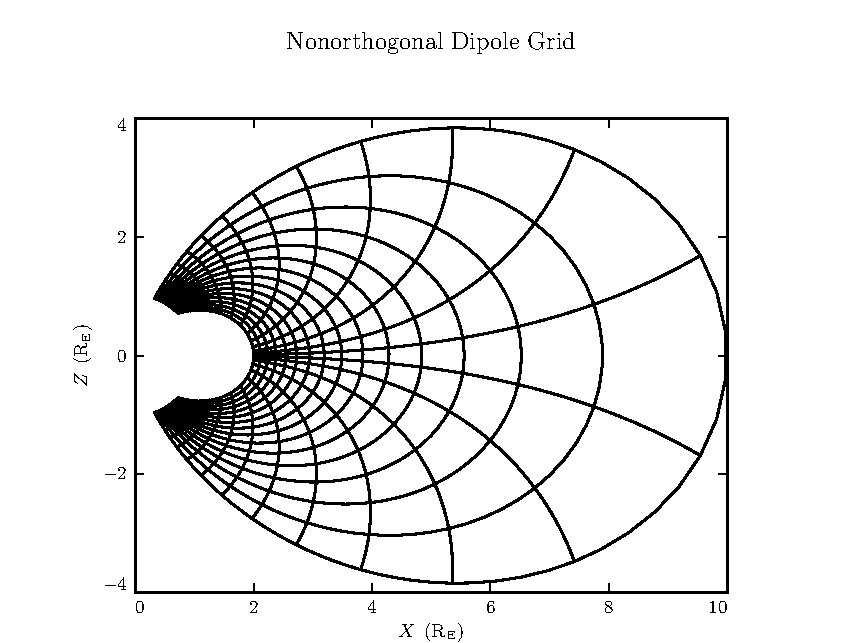
\includegraphics[width=\textwidth]{figures/grid.pdf}
    \caption[Nonorthogonal Dipole Grid]{
      The model's nonorthorthogonal dipole grid. Every fifth point is shown in each direction. The high concentration of grid points near Earth's equator is a consequence of the coordinate system, which converges at the equatorial ionosphere. 
    }
    \label{fig_grid}
\end{figure}

The simulation's time step is set based on the grid spacing. As is the convention, \dt is set to match the smallest \Alfven zone crossing time, scaled down by a Courant factor (typically 0.1). It bears noting that the smallest crossing time need not correspond to the smallest zone; recall from \cref{fig_va} that the \Alfven speed is very high in the Ionospheric \Alfven Resonator. 

\todo{Do we need a citation for how time steps are set based on crossing times? }

% =============================================================================
% =============================================================================
% =============================================================================
\section{Maxwell's Equations}
  \label{sec_eqns}

\todo{Introduce \farlaw and \amplaw, respectively, after using Kirchhoff's formulation of \ohmlaw ($\vec{J} = \tensor{\sigma} \cdot \vec{E}$) to eliminate explicit curl dependence... which will be revisited in \cref{ch_inertia}. }
\begin{align}
  \label{def_eqns}
  \ddt \vec{B} &= - \curl{E} &
  \tensor{\epsilon} \cdot \ddt \vec{E} &= \frac{1}{\mu_0} \curl{B} - \tensor{\sigma} \cdot \vec{E}
\end{align}

% -----------------------------------------------------------------------------
% -----------------------------------------------------------------------------
% -----------------------------------------------------------------------------
\subsection{Linearization and Optimization}
  \label{sec_optimization}

\todo{Leapfrog grid (for which Waters\cite{waters_2013} cites Taflove and Hagness, an electrodynamics textbook). Talk about the grid parity as well as the offset in time. }

%\begin{align}
%  \label{def_assign}
%  \begin{split}
%  \int_0^{\dt} \! dt \, \ddt \vec{B} &= - \displaystyle\int_0^{\dt} \! dt \, \curl{E} \\ 
%  \left. \vec{B} \right|_{\dt} - \left. \vec{B} \right|_0 &= \left. - \dt \, \curl{E} \right|_{ \frac{\dt}{2} } \\
%  \vec{B} &\assign \vec{B} - \dt \, \curl{E}
%  \end{split}
%\end{align}

\todo{Precomputation of coefficients. }

\todo{Curl shorthand, \vec{C} and \vec{F}. Recalling \cref{jacobian}, }
\begin{align}
  \label{def_curls}
  C^i & = \frac{ \varepsilon^{ijk} }{\jac} \dd{\lysakj} E_k &
  F^i & = \frac{ \varepsilon^{ijk} }{\jac} \dd{\lysakj} B_k
\end{align}

\todo{OpenMP. }

\todo{Keeping only covariant field components and contravariant curl components, since we only use contravariant coordinates. }

% -----------------------------------------------------------------------------
% -----------------------------------------------------------------------------
% -----------------------------------------------------------------------------
\subsection{Magnetic Fields}
  \label{sec_b}

Taking the shorthand introduced in \cref{def_curls}, \farlaw can simply be written: 
\begin{align}
  \label{farlaw_ijk}
  \ddt B^i &= - C^i
\end{align}

Writing each component out explicitly, and using the metric tensor (per \cref{metric}) to eliminate contravariant magnetic field components, \cref{farlaw_ijk} becomes:
\begin{align}
  \label{farlaw_final}
  \begin{split}
  B_1 &\assign B_1 - g_{11} \, \dt \, C^1 - g_{13} \, \dt \, C^3 \\
  B_2 &\assign B_2 - g_{22} \, \dt \, C^2 \\
  B_3 &\assign B_3 - g_{31} \, \dt \, C^1 - g_{33} \, \dt \, C^3
  \end{split}
\end{align}

Note that the \assign operator is used in \cref{farlaw_final} to indicate assignment, rather than equality. Terms on the left are new, while those on the right are old. 

% -----------------------------------------------------------------------------
% -----------------------------------------------------------------------------
% -----------------------------------------------------------------------------
\subsection{Electric Fields}
  \label{sec_e}

In \amplaw (per \cref{def_eqns}), the time derivative of the electric field depends on the electric field itself. As a result, it's best approached with integrating factors. 

To briefly 








Since \amplaw (\cref{def_eqns}) expresses the electric field time derivative in terms of the electric field itself, it must be solved with integrating factors. 


Noting the shorthand introduced in \cref{def_curls}, 




... \\

... \\

... \\

\amplaw, can be solved with integrating factors. From \cref{def_eqns}, 
\begin{align}
  \tensor{\epsilon} \cdot \ddt \vec{E} &= \frac{1}{\mu_0} \curl{B} - \tensor{\sigma} \cdot \vec{E}
\end{align}

The permittivity tensor can be trivially inverted. 
\begin{align}
  \label{amp_tensor}
  \lr{ \tensor{\Omega} + \tensor{ \mathbb{I} } \ddt } \cdot \vec{E} &= \tensor{v}^2 \cdot \vec{F}
\end{align}

Where $\tensor{ \mathbb{I} }$ is the identity tensor and in \x-\y-\z coordinates, 
\begin{align}
  \tensor{v}^2 &\equiv \frac{1}{\mz} \tensor{\epsilon}^{-1} = 
    \mmm{\va^2}{0}{0}
        {0}{\va^2}{0}
        {0}{0}{c^2}
  && \text{and} &
  \tensor{\Omega} &\equiv \tensor{\epsilon}^{-1} \cdot \tensor{\sigma} = 
    \mmm{ \frac{\sp}{\ep} }{ -\frac{\sh}{\ep} }{0}
        { \frac{\sh}{\ep} }{ \frac{\sp}{\ep} }{0}
        {0}{0}{ \frac{\sz}{\ez} } 
\end{align}

Using integrating factors, \cref{amp_tensor} gives
\begin{align}
  \vec{E} &\assign \exp \arg{ -\tensor{\Omega} \; \dt } \cdot \vec{E} + \dt \, \tensor{v}^2 \cdot \exp \arg{ -\tensor{\Omega} \; \tfrac{\dt}{2} } \cdot \vec{F}
\end{align}

\todo{Do we need to be careful here about the difference between a matrix and a tensor? }

The tensor exponential can be evaluated by considering the diagonal and off-diagonal terms separately. 
\begin{align}
  \tensor{\Omega} &= \tensor{\Omega}'
    + \frac{\sh}{\ep} 
    \mmm{0}{-1}{0}
        {1}{0}{0}
        {0}{0}{0} && \text{where} &
  \tensor{\Omega}' &=
    \mmm{ \frac{\sp}{\ep} }{0}{0}
        {0}{ \frac{\sp}{\ep} }{0}
        {0}{0}{ \frac{\sz}{\ez} }
\end{align}

Note that tensors are remarkably well-behaved when exponentiated\cite{hall_2015}. Because $\tensor{\Omega}'$ is diagonal, and thus the two commute,  
\begin{align}
  \exp \arg{ \tensor{T} } &= \displaystyle\sum_n \frac{1}{ n! } \tensor{T}^n &
  & \text{and} &
  \exp \arg{ \tensor{T} + \tensor{T}' } &= \exp \arg{ \tensor{T} } \exp \arg{ \tensor{T}' }
\end{align}

The off-diagonal terms collapse into sines and cosines, indicating a rotation about \z. 
\begin{align}
  \label{amp_final}
  \vec{E} &\assign \exp \arg{ -\tensor{\Omega}' \; \dt } \cdot \tensor{R}_z \arg{ \tfrac{-\sh \dt}{\ep} } \cdot \vec{E}
   + \dt \, \tensor{v}^2 \cdot \exp \arg{ -\tensor{\Omega}' \; \tfrac{\dt}{2} } \cdot \tensor{R}_z \arg{ \tfrac{-\sh \dt}{2 \ep} } \cdot \vec{F}
\end{align}

Where 
\begin{align}
  \tensor{R}_z \arg{\theta} &= 
  \mmm{\cos\theta}{-\sin\theta}{0}
      {\sin\theta}{\cos\theta}{0}
      {0}{0}{1}
\end{align}

The parallel term of term of \cref{amp_final} is simply
\begin{align}
  E_\parallel \assign E_\parallel \exp \arg{ \tfrac{- \sz \dt}{\ez} } + c^2 \dt F_\parallel \exp \arg{ \tfrac{- \sz \dt}{2 \ez} }
\end{align}

Or, in covariant terms, 
\begin{align}
  \label{amp_para}
  E_3 \assign E_3 \exp \arg{ \tfrac{- \sz \dt}{\ez} } + c^2 \dt \lr{ g_{31} F^1 + g_{33} F^3 } \exp \arg{ \tfrac{- \sz \dt}{2 \ez} }
\end{align}

For the ionospheric profiles and time steps employed by this model, $\frac{\sz \dt}{\ez}$ is never smaller than $10^3$. As a result, $\exp \arg{ \frac{- \sz \dt}{\ez} }$ is far too small to be stored in a double precision variable. That is, this simulation takes $E_\parallel$ (and, as a result, $E_3$) to be uniformly zero. 

This, obviously, precludes any discussion of parallel electric fields or parallel currents. These topics are revisited in \cref{ch_inertia}. 

Not unrelatedly, recalling the definition of the plasma frequency and parallel conductivity from \cref{def_basics}, $\frac{\sz}{\ez}$ can also be written $\frac{\op^2}{\nu}$. 

The plasma frequency is very fast. 

The perpendicular components of \cref{amp_final}, mapped from the physical basis to the contravariant basis (per \cref{def_xyz_directions}) to the covariant basis (per \cref{metric}), give
\begin{alignat}{6}
  \label{e1_final}
  & E_1 + \frac{ g^{13} }{ g^{11} } && E_3 \assign &&   && E_1 && \cos \arg{ \tfrac{- \sh \dt}{\ep} } \exp \arg{ \tfrac{- \sp \dt}{\ep} } &&  \notag \\
  &                                 &&             && + && E_2 && \sin \arg{ \tfrac{- \sh \dt}{\ep} } \exp \arg{ \tfrac{- \sp \dt}{\ep} } &&  \sqrt{ \frac{ g^{22} }{ g^{11} } } \notag \\
  &                                 &&             && + && E_3 && \cos \arg{ \tfrac{- \sh \dt}{\ep} } \exp \arg{ \tfrac{- \sp \dt}{\ep} } &&  \frac{ g^{13} }{ g^{11} } \\
  &                                 &&             && + && F^1 && \cos \arg{ \tfrac{- \sh \dt}{2\ep} } \exp \arg{ \tfrac{- \sp \dt}{2\ep} } &&  \frac{\va^2 \dt}{ g^{11} } \notag \\
  &                                 &&             && + && F^2 && \sin \arg{ \tfrac{- \sh \dt}{2\ep} } \exp \arg{ \tfrac{- \sp \dt}{2\ep} } &&  \frac{\va^2 \dt}{ \sqrt{ g^{11} g^{22} } } \notag \\
  \intertext{and}
  \label{e2_final}
  & && E_2 \assign && - && E_1 && \sin \arg{ \tfrac{- \sh \dt}{\ep} } \exp \arg{ \tfrac{- \sp \dt}{\ep} } &&  \sqrt{ \frac{ g^{11} }{ g^{22} } } \notag \\
  & &&             && + && E_2 && \cos \arg{ \tfrac{- \sh \dt}{\ep} } \exp \arg{ \tfrac{- \sp \dt}{\ep} } &&  \notag \\
  & &&             && - && E_3 && \sin \arg{ \tfrac{- \sh \dt}{\ep} } \exp \arg{ \tfrac{- \sp \dt}{\ep} } &&  \frac{ g^{13} }{ \sqrt{ g^{11} g^{22} } } \\
  & &&             && - && F^1 && \sin \arg{ \tfrac{- \sh \dt}{2\ep} } \exp \arg{ \tfrac{- \sp \dt}{2\ep} } &&  \frac{\va^2 \dt}{ \sqrt{ g^{11} g^{22} } } \notag \\
  & &&             && + && F^2 && \cos \arg{ \tfrac{- \sh \dt}{2\ep} } \exp \arg{ \tfrac{- \sp \dt}{2\ep} } &&  \frac{\va^2 \dt}{ g^{22} } \notag
\end{alignat}

The $E_3$ terms can be ignored at present, but \cref{ch_inertia} references back to them. 















% =============================================================================
% =============================================================================
% =============================================================================
\section{Driving}
  \label{sec_driving}

If no energy is added, the simulation is pretty boring. Everything just stays zero. 

% -----------------------------------------------------------------------------
% -----------------------------------------------------------------------------
% -----------------------------------------------------------------------------
\subsection{Outer Boundary Compression}

Driving from the outer boundary is the traditional way to do it. 

\todo{Cite and briefly explain past work done with compressional driving. }

As discussed in \cref{sec_math_implications}, \Alfven waves become guided when the azimuthal modenumber is large. The energy all stays close to the outer boundary. No field line resonances of significant strength are created within the magnetosphere. 

\todo{Should the model be presented first, or the dispersion relation? It's natural to talk about the ionospheric profiles when presenting the model, which the dispersion relation relies upon. But it's convenient, here, to be able to talk about how \Alfven waves become guided at large \azm. That probably means that the math should go first, and the ionospheric profiles should be squeezed in somewhere earlier. }

\begin{figure}[H]
    \centering
    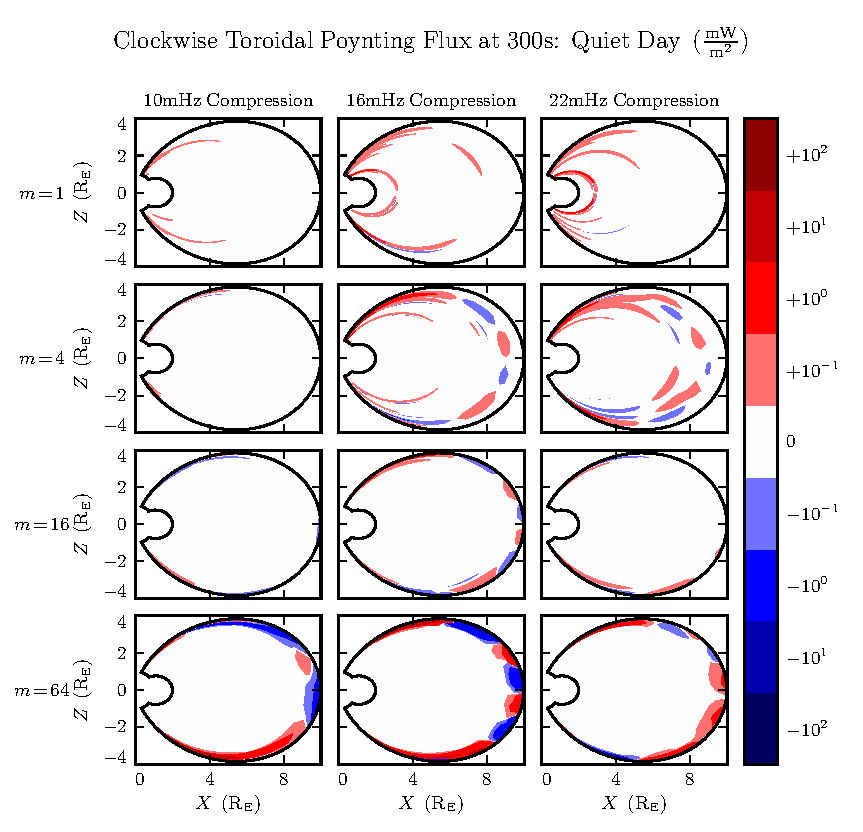
\includegraphics[width=\textwidth]{figures/Stor_B_2.pdf}
    \caption[Decreasing Penetration with Increasing Modenumber]{
      When the azimuthal modenumber is small, energy delivered through compression of the outer boundary is able to propagate across field lines and stimulate field line resonances in the inner magnetosphere. However, as modenumber increases, \Alfven waves become increasingly guided. As a result, energy delivered at the outer boundary cannot penetrate to the inner magnetosphere. Note that the large values on the bottom row should be taken with a grain of salt; it's not clear that the simulation is reliable when waves are continuously forced against the boundary. 
    }
    \label{fig_Stor_B_2}
\end{figure}

Compressional driving is applied by setting the value of $B_3$ at the outer boundary. 

A compression might reasonably be expected to drive waves with long azimuthal wavelengths. However, there is some indication that waves with short azimuthal wavelength can be driven as well, such as through Kelvin-Helmholtz interactions. 

\todo{Find this claim again and cite it. }

% -----------------------------------------------------------------------------
% -----------------------------------------------------------------------------
% -----------------------------------------------------------------------------
\subsection{Ring Current Modulation}

Pc4 pulsations with high azimuthal modenumber are known to be driven from within the magnetosphere, such as through drift-resonant interactions with energetic radiation belt and ring current particles. 

\todo{Cite. }

\todo{Careful with units! Is this nT, or nT/mHz, or what? }

Substorm injection can cause localized ring current behavior. 

\todo{UNH was looking at this at AGU. Check if they have published yet. }

During geomagnetically active times, the ring current is a dynamic region. It's easy to imagine localized perturbations. 

It's difficult to estimate how large such perturbations might be. The following is a kludgey estimate. 

\begin{figure}[H]
    \centering
    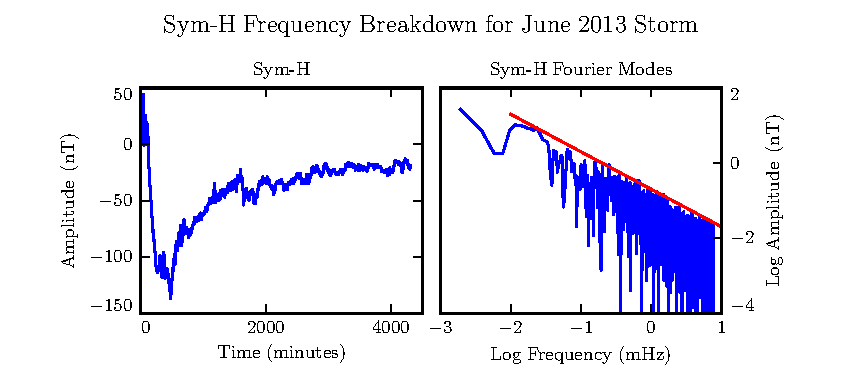
\includegraphics[width=\textwidth]{figures/symh.pdf}
    \caption[Sym-H Fourier Components for June 2013 Storm ]{
      The Sym-H storm index (from NASA CDAWeb\cite{nasa_cdaweb}) measures magnetic perturbations on Earth's surface due to ring current activity. It is measured once per minute, so Fourier amplitudes in the Pc4 range cannot be measured directly. However, they can be inferred by fitting the pink noise. The red line shows a fit to the top of the distribution, $\sim$ \SI{e-2}{\nano\tesla} $\lr{ \frac{ \SI{20}{\mHz} }{f} }$. 
    }
    \label{fig_symh}
\end{figure}

Sym-H is like Dst, but with greater time resolution. 

The noise suggests that a Fourier component with a period of about \SI{1}{\minute} could have an amplitude around \SI{e-2}{\nano\tesla}. 

If the driving is delivered at $L=5$, with a standard deviation of \SI{0.5}{\RE} in the radial direction and \SI{5}{\degree} angularly, that corresponds to a current density on the order of \SI{e-4}{\uA/\meter\squared}. This comes from approximating the ring current as a ring of current. Of course, Sym-H is measured at Earth's surface, not at the center of the ring; this gives a geometric factor of about two. 

\todo{What electric field magnitude does this correspond to? }

Current driving is applied by adding an additional current term. \amplaw becomes
\begin{align}
  \tensor{\epsilon} \cdot \ddt \vec{E} &= \frac{1}{\mu_0} \curl{B} - \tensor{\sigma} \cdot \vec{E} - \vec{J}_{drive}
\end{align}

And this driving term is absorbed into the curl by revising \cref{def_curls} from $\vec{F} \equiv \curl{B}$ to $\vec{F} \equiv \curl{B} - \vec{J}_{drive}$. (As a result, \cref{e1_final,e2_final} do not change.)

Notably, Sym-H is a global quantity; it's not ideally suited for making estimates of localized inhomogeneity. 

Furthermore, Sym-H has a time resolution of \SI{1}{\minute}. It can hardly be said to carry information about oscillations at frequencies of less than two minutes. 

Sym-H gives no way to estimate azimuthal modenumber. That's based on Pc4 observations. Dai\cite{dai_2015} observed modenumbers approaching \num{100}. 

A kludgey estimate is better than no estimate. 

% =============================================================================
% =============================================================================
% =============================================================================
\section{Boundary Conditions}
  \label{sec_bcs}

The grid can't go on forever. There have to be special cases at the edges. 


% -----------------------------------------------------------------------------
% -----------------------------------------------------------------------------
% -----------------------------------------------------------------------------
\subsection{Parity and Interpolation}

Computation takes place on a staggered grid. 

Field values are offset to ensure that most differences are centered. For example, $\ddt B_2$ depends on $\dd{\lysakx} E_3$ and $\dd{\lysakz} E_1$. If $B_2$ is defined at even $i$, $E_3$ is defined at odd $i$, so that $B_2$ is defined on the same grid points as $\frac{ E_3 \lrb{i+1} - E_3 \lrb{i-1} }{ \lysakx \lrb{i+1} - \lysakx \lrb{i-1} }$. 

\todo{Make sure the example uses the currect parities. }

\todo{Find a citation for the wigglies that occur if field values are defined on all grid points, due to the weak coupling. This problem is apparently well-known. }

Values are sometimes needed off-parity. $E_1$ and $E_2$ are not defined at the same grid locations, but they are coupled directly by the Hall conductivity. And $B_1$ and $B_3$ are coupled by the non-orthogonality of the grid. When off-parity values are needed, they are interpolated from their neighbors. 

Differentiation and interpolation are good to second order on the nonuniform grid. Like the coefficients for Maxwell's equations, differentiation and interpolation weights are computed during setup to save time during iteration. 

Electric fields go to zero at the innermost and outermost field lines (Dirichlet boundary conditions). Magnetic fields have zero derivative (Neumann boundary conditions). For components not defined at the exact boundary, these rules are applied when differentiating or interpolating; they set the effective value just outside the grid. 

These boundary conditions can in principle cause nonphysical reflection at the boundary. In practice, that is not an issue. Wave activity is concentrated well away from the boundaries. In fact, reversing the Dirichlet and Neumann boundary conditions has little effect. 

(Of course, an inconsistent boundary condition -- like using the same boundary condition for a field and its derivative -- causes instability.)

% -----------------------------------------------------------------------------
% -----------------------------------------------------------------------------
% -----------------------------------------------------------------------------
\subsection{Coupling to the Atmosphere}

Conditions at the ionospheric boundaries are set by coupling to the atmosphere. This also allows the computation of ground fields. 

It's reasonable to approximate the atmosphere as a perfect insulator, giving $\curl{B}=0$. Combining with $\div{B}=0$ per Maxwell's equations, ensures the existence of a scalar magnetic potential $\Psi$ such that $\vec{B}=\grad{\Psi}$ and $\Psi$ satisfies Laplace's equation, $\nabla^2 \Psi = 0$. 

Laplace's equation can be solved analytically; in spherical coordinates, the solutions are spherical harmonics. However, a numerical solution is preferrable to ensure orthonormality on a discrete (and incomplete -- there are no grid points at the poles or equator) grid. After separating out the radial and azimuthal dependence in the usual way, the latitudinal component of Laplace's equation (in terms of $s \equiv - \sin^2 \theta$) is
\begin{align}
  \label{laplace}
  \lr{ 4 s^2 + 4s } \frac{d^2}{ds^2} Y_\ell + \lr{ 4 + 6 s } \frac{d}{ds} Y_\ell - \frac{\azm^2}{s} Y_\ell &= \ell \lr{ \ell + 1 } Y_\ell
\end{align}

Using centered differences to express the derivatives, \cref{laplace} is a system of linear equations, one per field line. It can be solved numerically for eigenvalues $\ell \lr{\ell + 1}$ and eigenvectors (harmonics) $Y_\ell$. In terms of those harmonics, and noting that the model uses a fixed azimuthal modenumber \azm, $\Psi$ between $R_E$ and $R_I$ can be expressed
\begin{align}
  \label{psi_expansion}
  \Psi \arg{r, \theta, \phi} &= \displaystyle\sum_\ell \lr{ \alpha_\ell \, r^\ell + \beta_\ell \, r^{-\ell - 1} } Y_\ell \arg{\theta} \exp \arg{i \azm \phi}
\end{align}

\todo{Conductivity tensor at the ionosphere comes from\cite{lysak_2004}. }

As a boundary condition for $\Psi$, Earth's crust is assumed to be a perfect conductor, forcing the magnetic field at the boundary to be perfectly horizontal. That is, $B_r = \dd{r} \Psi = 0$. Then, noting that the harmonics $Y_\ell$ are orthonormal (so each term of the sum must be zero), 
\begin{align}
  \label{beta_solution}
  \beta_\ell &= \frac{\ell}{\ell + 1} R_E^{2 \ell + 1} \alpha_\ell
\end{align}

Note that the explicit $\phi$ dependence has been dropped. The entire simulation shares a fixed modenumber, so it's sufficient to find $\Psi$ at $\phi=0$. 

At the top of the atmosphere, the radial magnetic field is again used as a boundary condition, this time to compute the weights $\alpha_\ell$. 

\todo{Something something thin horizontal current sheet at $R_I$. }

Taking the shorthand $\lambda_I \equiv \frac{R_E}{R_I} \sim \num{0.975}$
\begin{align}
  B_r &= \displaystyle\sum_\ell \ell \, \alpha_\ell \, R_I^{\ell-1} \, \lr{ 1 - \lambda_I^{2 \ell - 1} } Y_\ell
\end{align}

\todo{Settle on good notation for taking the inner product of harmonics. It's a vector in the sense that it's a one-dimensional array of values, but not in the physical sense. Indexing -- $B_r\lrb{i}$ -- also seems awkward. }

The sum can be collapsed by ``integrating" over a harmonic. The inverse harmonics are obtained by inverting the eigenvector matrix. Then $Y_\ell \cdot Y_{\ell'}^{-1} = \delta_{\ell \ell'}$ by construction. 
\begin{align}
  \label{alpha_solution}
  \alpha_\ell &= \frac{ 1 }{\ell \, R_I^{\ell-1} } \frac{ B_r \cdot Y_\ell^{-1} }{ 1 + \lambda_I^{2 \ell + 1} }
\end{align}

Combining \cref{psi_expansion,beta_solution,alpha_solution} allows the expression of $\Psi$ at the top and bottom of the atmosphere as a linear function of the radial magnetic field at the boundary. 
\begin{align}
  \label{psi_final}
  \begin{split}
  \Psi_E &= \displaystyle\sum_\ell Y_\ell \; \frac{R_I}{\ell} \frac{ \frac{2 \ell - 1}{\ell - 1} \lambda^\ell }{ 1 - \lambda_I^{2 \ell + 1} } B_r \cdot Y_\ell^{-1} \\
  \Psi_I &= \displaystyle\sum_\ell Y_\ell \; \frac{R_I}{\ell} \frac{ 1 + \frac{\ell}{\ell - 1} \lambda_I^{2 \ell + 1} }{ 1 - \lambda_I^{2 \ell + 1} } B_r \cdot Y_\ell^{-1}
  \end{split}
\end{align}

Magnetic fields are evaluated from $\Psi$ per 
\begin{align}
  B_1 &= \dd{\lysakx} \Psi &
  B_2 &= \dd{\lysaky} \Psi
\end{align}

Note that $B_1$ and $B_2$ are horizontal; per \cref{def_rqf_directions}, they are proportional to $B_\theta$ and $B_\phi$ respectively. 

At the ground, field values are purely output. 

Horizontal magnetic field values at the top of the ionosphere, on the other hand, are used as boundary conditions. Assuming there is no vertical component to the ionospheric current sheet, the electric field values at the ionospheric edge of the grid are dictated by the jump in horizontal magnetic field between the bottom of the grid and the top of the atmosphere. 
\begin{align}
  \mz \, \tensor{\Sigma} \cdot \vec{E} &= \left. \displaystyle\lim_{\dr \rightarrow 0} \, \hat{r} \! \times \! \vec{B} \, \right|^{R_I + \dr}_{R_I - \dr}
\end{align}

\todo{Bob's citations for the ionospheric jump conditions: Fujita and Tamao 1988, Yosikawa and Itonaga 1996, 2000, Lysak and Song 2001, Sciffer and Waters 2002. It basically comes from integrating \amplaw, so half a dozen citations seems like overkill. }

The harmonic breakdown of $\Psi$ also allows for the calculation of how much energy is leeched by the atmosphere. 
\begin{align}
  B_r &= \dd{r} \Psi &
  B_\theta &= \frac{1}{r} \dd{\theta} \Psi &
  B_\phi &= \frac{1}{r \sin\theta} \dd{\phi} \Psi
\end{align}  

\todo{Plug \cref{psi_expansion,beta_solution} into these expressions, then that into $u = \frac{1}{2 \mz} \left| \vec{B} \right|^2 $, then integrate from $R_E$ to $R_I$ and in angle. }







% =============================================================================
% =============================================================================
% =============================================================================
\section{Ionospheric Profile}
  \label{sec_ionos}

\todo{Just refer back to the profiles we show in chapters 1 and 2(?). We don't need to explain how to read in a profile and map it to a grid. }

The ionospheric profiles used in this model are based on values tabulated in the Appendix B of Kelley's book\cite{kelley_1989}. They were adapted by Lysak\cite{lysak_2013} to take into account the effect of the magnetosphere's latitude-dependent density profile. 

Mean molecular mass of \SI{28}{\amu} at \SI{100}{\km}, \SI{16}{\amu} around \SI{400}{\km}, down to \SI{1}{\amu} above \SI{1400}{\km}. 

Simulations are carried out using four profiles: active day, quiet day, active night, quiet night. 

Profiles are static for the duration of a simulation. Even so-called ultra low frequency waves are still much faster than convective timescales. 

\todo{Come up with a characteristic convective timescale or two, and cite it. }

% -----------------------------------------------------------------------------
% -----------------------------------------------------------------------------
% -----------------------------------------------------------------------------
\subsection{Conductivity}

The effects of mean molecular mass on conductivity are computed per the usual definitions. 
\begin{align}
  \sp &= \displaystyle\sum_s \frac{n_s q_s^2}{m_s} \frac{\nu_s}{\nu_s^2 + \Omega_s^2} &
  \sh &= -\displaystyle\sum_s \frac{n_s q_s^2}{m_s} \frac{\Omega_s}{\nu_s^2 + \Omega_s^2} &
  \sz &= \displaystyle\sum_s \frac{n_s q_s^2}{m_s \nu_s}
\end{align}

Each profile is resolved to an altitude of about $\SI{e4}{\km}$, and include well-resolved $E$, $F_1$, and $F_2$ layers. 

\todo{Talk about the ionospheric layers, probably in the introduction. }

\begin{figure}[H]
    \centering
    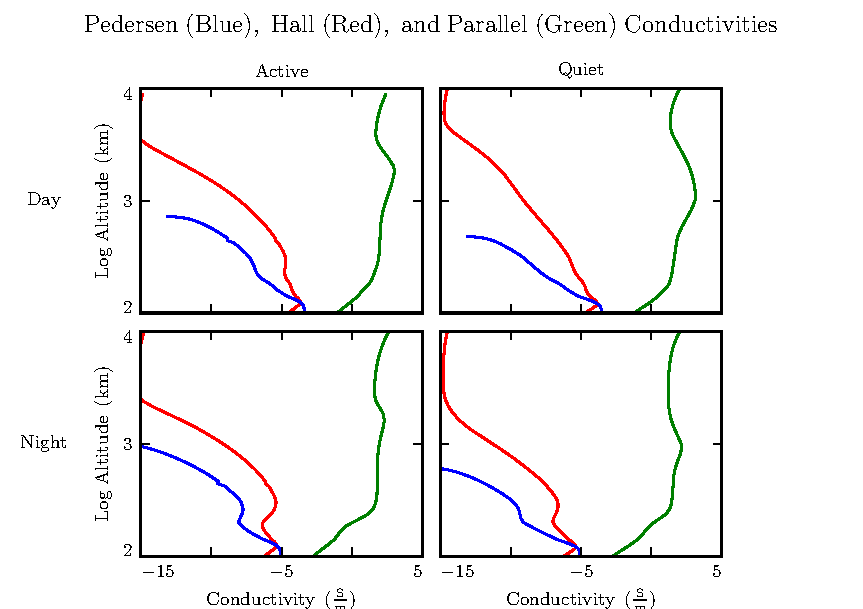
\includegraphics[width=\textwidth]{figures/sigma.pdf}
    \caption[Ionospheric Conductivity Profiles]{
      Ionospheric conductivity profiles, adapted by Lysak\cite{lysak_2013} from Appendix B of Kelley's textbook\cite{kelley_1989}. 
    }
    \label{fig_sigma}
\end{figure}

\todo{What is the height-interated conductivity for each profile? }

% -----------------------------------------------------------------------------
% -----------------------------------------------------------------------------
% -----------------------------------------------------------------------------
\subsection{\Alfven Speed}

The \Alfven speed is computed from Kelley's low-density profile, modified to take into account the local density. The density, in turn, is the sum of a plasmaspheric profile and a high-latitude auroral profile. 
\begin{align}
  \ep &= \text{(low-density tabulated value)} + \frac{ n \bar{m} }{B_0^2}
\end{align}

\todo{What's a clean way of showing the low-density \ep that we read in? }

\todo{Does Kelley list the electric constant or the \Alfven speed? }

Where $\bar{m}$ is the ambient mean molecular mass and $B_0$ is the zeroth-order magnetic field strength, $B_0 = \SI{3.11e4}{\nano\tesla} \lr{ \frac{R_E}{r} }^3 \sqrt{ 1 + 3 \cos^2 \theta }$. Note that \SI{3.11e4}{\nano\tesla} is the value of the Earth's magnetic field at the equator on Earth's surface. 

\todo{Cite this number? Jesse just says it's a ``representative'' number. He uses \SI{30}{\micro\tesla}. }

\begin{figure}[H]
    \centering
    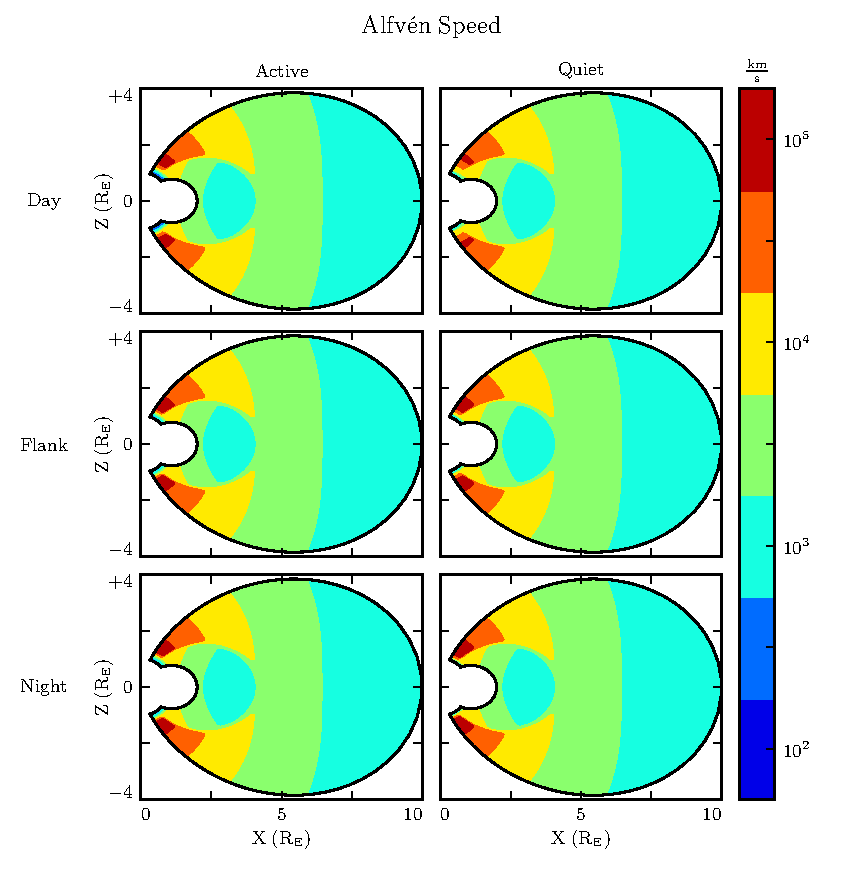
\includegraphics[width=\textwidth]{figures/va.pdf}
    \caption[\Alfven Speed Profiles]{
      \Alfven speed profiles, adapted by Lysak\cite{lysak_2013} from Appendix B of Kelley's textbook\cite{kelley_1989}. 
    }
    \label{fig_va}
\end{figure}

\todo{Above the profile, Bob scales the value that's read in as $r^5$ or something. Is there a citation for that? }

The \Alfven speed is then computed per $\va^2 \equiv \frac{1}{\mz \ep}$. 

\begin{figure}[H]
    \centering
    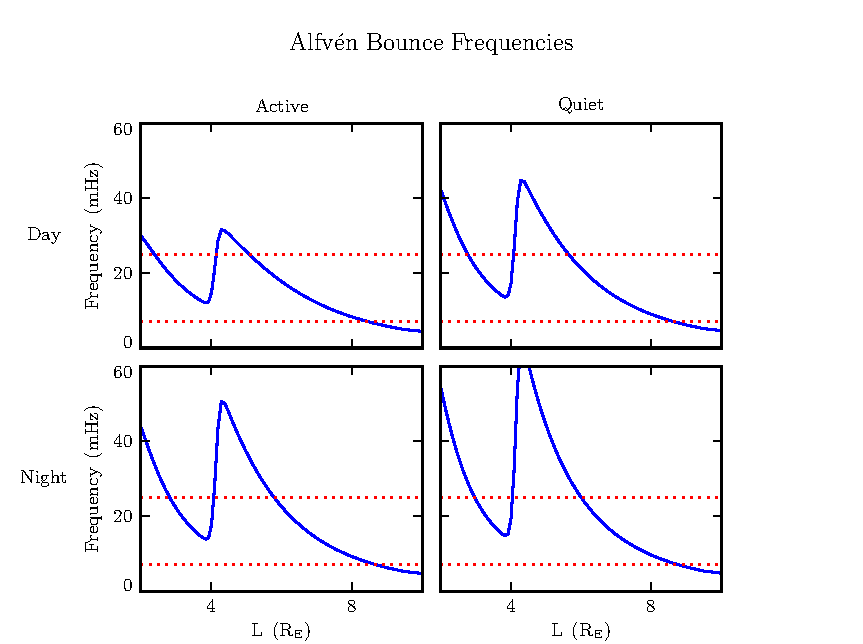
\includegraphics[width=\textwidth]{figures/fa.pdf}
    \caption[\Alfven Bounce Frequency Profiles]{
      \Alfven bounce frequency profiles, computed by integrating the the \Alfven speed back and forth over a field line. $f_A = \lrb{ \oint \frac{dz}{v_A} }^{-1}$. Dotted lines indicate the Pc4 frequency range, \SIrange{7}{25}{\mHz}. In each profile, the effect of the plasmapause is clearly visible, centered at $L=4$. Field lines just inside and just outside the plasmapause appear susceptible to resonance in the Pc4 band. 
    }
    \label{fig_fa}
\end{figure}

\todo{Talk about how the size of the plasmasphere can be adjusted, and \SI{4}{\RE} is just a typical value. }

\todo{Explain how the \Alfven speed constrains the time step. }




